% https://www.palass.org/sites/default/files/media/publications/for_authors/ITA_2016_v1.pdf
% Abstract < 300w ---> OK
% Keywords < 6 ---> OK

\documentclass[12pt,letterpaper]{article}
\usepackage{natbib}

%Packages
\usepackage{fixltx2e}
\usepackage{textcomp}
\usepackage{fullpage}
\usepackage{float}
\usepackage{latexsym}
\usepackage{url}
\usepackage{epsfig}
\usepackage{graphicx}
\usepackage{amssymb}
\usepackage{amsmath}
\usepackage{mathtools}
\usepackage{bm}
\usepackage{array}
\usepackage[version=3]{mhchem}
\usepackage{ifthen}
\usepackage{caption}
\usepackage{hyperref}
\usepackage{amsthm}
\usepackage{amstext}
\usepackage{enumerate}
\usepackage[osf]{mathpazo}
\usepackage{dcolumn}
\usepackage{lineno}
\usepackage{pdflscape}
\usepackage{xcolor}
\usepackage{color,soul}

\DeclarePairedDelimiter\abs{\lvert}{\rvert}%
\DeclarePairedDelimiter\norm{\lVert}{\rVert}%
\newcolumntype{d}[1]{D{.}{.}{#1}}

\pagenumbering{arabic}


%Pagination style and stuff
\linespread{2}
\raggedright
\setlength{\parindent}{0.5in}
\setcounter{secnumdepth}{0} 
\renewcommand{\section}[1]{%
\bigskip
\begin{center}
\begin{Large}
\normalfont\scshape #1
\medskip
\end{Large}
\end{center}}
\renewcommand{\subsection}[1]{%
\bigskip
\begin{center}
\begin{large}
\normalfont\itshape #1
\end{large}
\end{center}}
\renewcommand{\subsubsection}[1]{%
\vspace{2ex}
\noindent
\textit{#1.}---}
\renewcommand{\tableofcontents}{}
%\bibpunct{(}{)}{;}{a}{}{,}

%---------------------------------------------
%
%       START
%
%---------------------------------------------

\begin{document}
%Running head
\begin{flushright}
Version dated: \today
\end{flushright}

\bigskip
\noindent RH: Characters correlation
\bigskip
\medskip
\begin{center}
\noindent{\Large \bf Influence of morphological character correlation on phylogenetic tree inference}
\bigskip

\noindent {\normalsize \sc Thomas Guillerme$^{1,2,*}$, Abigail I. Pastore$^{1}$, and Martin D. Brazeau$^{2,3}$}\\
% Abigail I. Pastore$^{1}$
\noindent {\small \it 
$^1$School of Biological Sciences, University of Queensland, St. Lucia, Queensland, Australia.\\
$^2$Imperial College London, Silwood Park Campus, Department of Life Sciences, Buckhurst Road, Ascot SL5 7PY, United Kingdom.\\
$^3$Department of Earth Sciences, Natural History Museum, Cromwell Road, London, SW75BD, United Kingdom.\\}

% TODO: change the affiliations


\end{center}
\medskip
\noindent{*\bf Corresponding author.} \textit{guillert@tcd.ie}\\ 
\vspace{1in}

%Line numbering
\modulolinenumbers[1]
\linenumbers

%---------------------------------------------
%
%       ABSTRACT
%
%---------------------------------------------

% SystBiol
% Palaeobiology
% JEB
% Biological Journal of the Linnean Society
% Royal Society Open Science - but rewriting needed (more story style)
% Palaeontology


% CITE: https://academic.oup.com/sysbio/article/68/2/267/5145070#130574594

% Mention Hamming distance rather than Gower?

\newpage
\begin{abstract}
Phylogenetic analysis algorithms assume character independence - a condition generally acknowledged to be violated by morphological data.
Correlation between characters can originate from intra-organismal features, \textcolor{blue}{evolutionary dependence} or forced by particular character-state coding schemes.
Although the two first sources can be investigated by biologists \textit{a posteriori} and the third one can be diminished \textit{a priori} with careful character coding, phylogenetic software do not distinguish between any of them.
In this study, we use a metric of raw character difference as a proxy for character correlation.
Using thorough simulations, we test the effect of increasing or decreasing character differences on tree topology.
Overall, we found a negative effect of reducing character correlations on recovering the correct topology.
This means that datasets with low correlation between characters will make it more complicated to estimate a correct topology.
However, this effect is less important for matrices with a small number of taxa (25 in our simulations) where reducing or increasing character correlation is not more effective in getting the expected topology than randomly drawing characters.
Furthermore, in bigger matrices (350 characters), the inference method has a strong effect with Bayesian trees being consistently less affected by character correlation than maximum parsimony trees.
These results suggest that ignoring the problem of character correlation or independence can often impact topology in phylogenetic analysis.
However, encouragingly, they also suggest that, unless correlation is actively maximised or minimised, probabilistic methods can easily accommodate for a random correlation between characters.

\end{abstract}

\noindent (Keywords: Character difference, correlation, topology, Bayesian, maximum parsimony)\\

\vspace{1.5in}

\newpage 

%---------------------------------------------
%
%       INTRODUCTION
%
%---------------------------------------------
\section{Introduction}
The last two decades have witnessed a resurgence of interest in the use of morphological character data in phylogenetic studies.
This owes in large part to the advent of new models, methods and software \citep{lewisa2001,ronquista2012,Ronquist2012mrbayes,heath2014fossilized} and the use of fossils to undertake at least partial reconstructions of phylogenetic trees, especially where ancestral states reconstructions or absolute calibrations of divergence times are necessary.
While there is a general appreciation of the limits of morphological data, they are frequently dismissed without any investigations into their statistical properties. %MB: I think there are a few classic papers we could cite here. The dismissal tends to arise with the same 'workflow': calculate a molecular tree; calculate a morphological tree; see that they are different; shit on the morphological tree because of this that and the other, but never bother to check if the data actually suggest these phenomena. TG: which ones?
As morphological data are likely to continue to play an extensive role in phylogenetic analysis,  %MB: cite Nature paper here. TG: which one?
it is essential to understand the circumstances under which morphological data might be expected to lead to erroneous phylogenetic inferences.
This opens up possibilities for analysing problematic datasets and possibly proposing new confidence measures in phylogenetic datasets.

The non-independence of large numbers of morphological characters is often cited in anticipation of problems with morphological data \cite[e.g.][]{Davalos01072014, ZouConvergence}.
The assumption of character independence is central to phylogenetic inference methods such as maximum likelihood and maximum parsimony \citep[e.g.][]{joysey1982problems,felsenstein1985phylogenies,lewisa2001,felsenstein2004inferring}.
Non-independence of characters implies that some suites of characters are expected to transform in highly correlated ways.
Not only does this violate the assumptions of phylogenetic analysis, but implies that if convergence has occurred in correlated sets of characters, then this would lead to spurious cladistic groupings.
Here we distinguish three different modes of forms of character correlation (described in more details in \citealt{wilkison1992ordered,wilkinson1995character,wilkinson1995coping}):

\begin{itemize}
    \item \textbf{Intra-organismal dependence:} this is the result of an intrinsic biological link between two characters.
    For example the occlusal surface of two opposing molars will be expected to directly covary.
 
    \item \textbf{Evolutionary dependence:} this is the result of sets of characters co-evolving. 
    For example, in vertebrates, axial elongation can be correlated to limb reduction with snake-like bodies evolving multiple times in numerous tetrapod lineages.

    \item \textbf{Logical dependence:} this is the results of researcher methodology for defining or/and coding discrete morphological characters \citep{Brazeau2011,simoes2017giant}.
    For example, two characters ``tail colour'' and ``tail length'' could be coded two times as an absence for a taxon with no tail \citep{wilkinson1995coping,BrazeauNA}.
    \textcolor{blue}{Note that there are a lot of alternative methodological choices for this example \citep[e.g. using inapplicable tokens; ][]{Brazeau2011} and that these choices affect results more or less depending on the estimation method (parsimony methods contrast with probabilistic methods were ancestral conditions are respectively fixed or not).}
\end{itemize}

\noindent Of course, the three sources of dependence can have an interaction: characters describing the left and right lower/upper molars will have induced dependence due to the modularity of the molars, their shared history and the duplicated coding.
Logical dependence, however, is easily distinguished prior to phylogenetic inference, while intra-organismal and evolutionary dependence are much harder to parse.
Meanwhile, the development of algorithms and software has not yet caught up with the need to deal with these interdependencies \citep{de2015parsimony,BrazeauNA}.
Intra-organismal dependence requires more detailed, often extremely time-consuming studies (possibly beyond the limits of available technology).
Evolutionary dependence itself requires the accurate resolution of a phylogenetic tree (but see useful methods from \citealt{Pagel1994} and \citealt{billet2019serial}), and is best determined by independent character sets.
\textcolor{blue}{The latter is commonly hard to get because of the nature of the data: some common types of data (e.g. fossil data) offer very few options of independent character sets and no biological datasets can really be independent.
It is also worth noting that the evolutionary and intra-organismal dependences induced correlations are by no means restricted to the use of discrete morphological data. In fact, by essence, these correlations appear to any type of data whether continuous (e.g. linear measurements or morphometric geometric measurements) or non-morphological (e.g. behaviour, or - much more commonly used - molecular data).}

\color{black}{Intra-organismal} and evolutionary dependences are inherent parts to Evo-Devo and macroevolutionary studies and best practices to avoid coding-induced dependences are commonly known and applied.
However, eventually, all these characters, whether they are independent or not are analysed through phylogenetic inference software that are blind to these distinctions.
If fact, what the software are confronted with is a two dimensional matrix problem that renders all morphological dependencies invisible.
The majority of phylogenetic algorithms cannot interpret character descriptions and state meanings, and instead must interpret discrete states as signifiers of shared similarity: for each characters, species are grouped if they have identical characters.
Therefore, character with the same number of states will have a chance of being correlated regardless of mode of form of character correlation.

\noindent How does character correlation really affect topology?
Although it has been tackled empirically (for morphological data \citealt{Davalos01072014}, and molecular data \citealt{ZouConvergence}), the question has never been explored through a thorough simulation framework.
Simulations can allow the design of datasets with controlled levels of correlation and for which the correct expected answer is known by design.
Furthermore, using simulations will allow drawing generalities on the effect of character correlation on phylogenetic inference in contrast to potential idiosyncrasies of empirical datasets.
Here we use a Hamming distance metric to measure the difference between characters (as a proxy for these three sources of correlation as interpreted by the software) and a protocol to modify discrete morphological matrices to increase or decrease the overall differences or similarities between characters.
We found that overall, there is a clear effect of character correlation on topology where a decrease in character correlation results in a decrease in the ability to recover the correct topology.
These results, however, vary greatly in magnitude depending on the size of matrix and the inference method used.

%---------------------------------------------
%
%       METHODS
%
%---------------------------------------------
\section{Methods}
To assess the effects of character correlation on the accuracy of phylogenetic inference we generated a series of matrices exhibiting different average correlation between characters (Fig.\ref{Fig:outline} - note that each step is described in more details below):
\begin{enumerate}
    \item \textbf{Simulating matrices}: \textcolor{blue}{using a randomly generated topology (the \textit{starting tree})} we simulated discrete morphological matrices with 25, 75 or 150 taxa, for 100, 350 or 1000 characters, hereafter called the \textcolor{blue}{\textit{unperturbed matrices}}.
    This step resulted in 9 matrices.

    \item \textcolor{blue}{\textbf{Inducing correlation}: To induce different levels of unpredicted correlation, we used the unperturbed matrices as the basis of a series of resampling manipulations that either enriched or depleted the matrix with correlated characters.
    We modified the matrices by running three types of bootstrapping methods (i.e. removing a set of characters by a set of remaining ones): 1) a classical bootstrap (randomly removing/replacing characters) as our null change in character correlation (hereafter, the \textit{randomised matrices}); 2) a biassed bootstrap towards correlation (removing/replacing the most different characters) to generate matrices with maximised correlation (the \textit{maximised correlation matrices}) and 3) a biassed bootstrap away from correlation (removing/replacing the least different characters) to generate the \textit{minimised correlation matrices} (i.e. with a minimised amount of correlation).}

    \item \textcolor{blue}{\textbf{Inferring topologies}: we inferred the topologies from the unperturbed, randomised, maximised correlation and minimised correlation matrices using both maximum parsimony and Bayesian inference. Hereafter, the resultant topologies are called the unperturbed, randomised, maximised correlation and minimised correlation trees.}

    \item \textcolor{blue}{\textbf{Comparing topologies}: finally, we compared the unperturbed tree to the trees recovered from analysis of the three different dataset types (randomised, maximised and minimised correlation) to measure the effect of character correlation on the recovered topology.}

\end{enumerate}
All steps were replicated 20 times and are described below in more detail.
\textcolor{blue}{Note that we compare to the topologies from the randomised, maximised and minimised correlation trees to the unperturbed tree rather than to the starting tree because differences with the starting tree can be due to other confounding factors which are out of the scope of this study (e.g. the algorithms used to simulate characters).}

\begin{figure}[!htbp]
\centering
   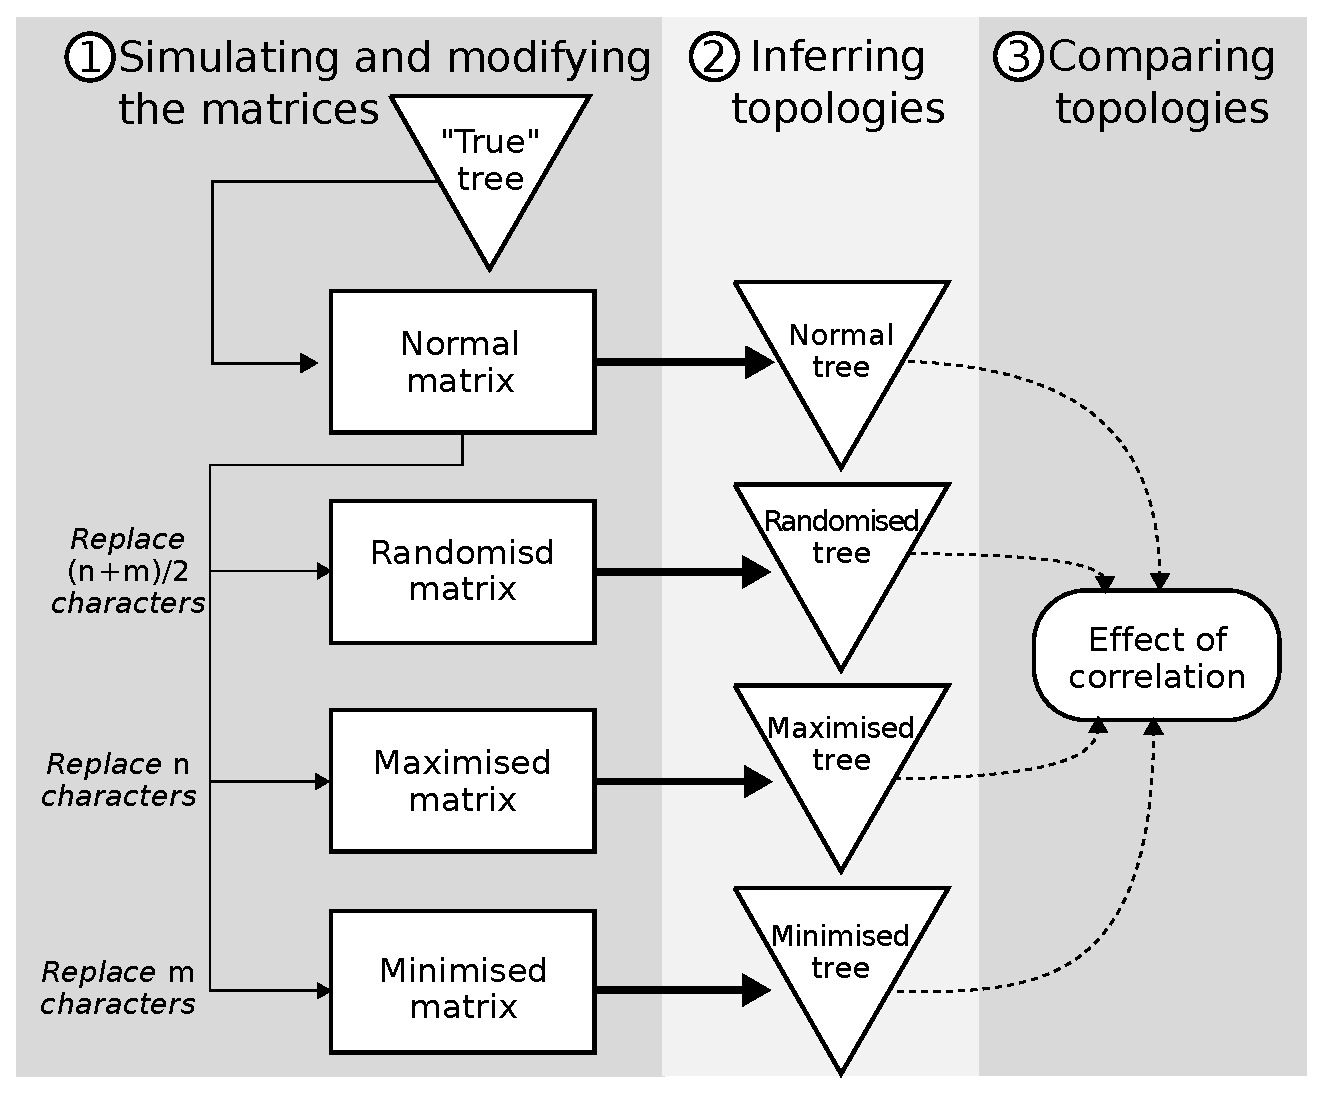
\includegraphics[width=0.9\textwidth]{outline.eps}
\caption{Outline of the simulation protocol: the first step includes both the simulation and the modification of the matrices (thin solid lines); the second step includes tree inference using maximum parsimony and Bayesian inference methods (thick solid lines); the third step includes comparing the resulting tree topologies (dashed lines). $n$ and $m$ corresponds to the number of characters with a character difference $<0.25$ and $>0.75$ respectively.}
\label{Fig:outline}
\end{figure}
''
\subsection{Simulating discrete morphological matrices}

To simulate the matrices we applied a protocol very similar to \cite{Guillerme2016146} using \texttt{R} \citep{R}.
First, we generate random birth-death trees with the birth ($\lambda$) and death ($\mu$) parameters sampled from a uniform $(0,1)$ distribution with $\lambda$ $>$ $\mu$ \citep[\texttt{diversitree} v0.9-8;][]{fitzjohndiversitree2012} and saving the trees after reaching either 25, 75 or 150 taxa (see supplementary material 3, Figs 1, 2 and 3).
For each tree, we arbitrarily set the outgroup to be the first taxon (alphabetically) thus effectively rooting the trees on this taxon.
These trees are hereafter called the \textcolor{blue}{\textit{starting trees}}.
We then simulated discrete morphological characters on the topology of these trees using the either of the two following models:
\begin{itemize}
    \item The ``morphological HKY-binary'' model \citep{OReilly20160081} which is an HKY model \citep{HKY85} with a random states frequency (sampled from a Dirichlet distribution $Dir(1,1,1,1)$) and using a transition/transvertion rate of $2$ \citep{douadycomparison2003} but where the purines (A,G) were changed into state $0$ and the pyrimidines (C,T) in state $1$.
    \textcolor{blue}{This allows the changes in character states to vary without specifying which change is more likely, hence expecting an equiprobable change in character state in all directions.}
    \item To generate more than binary states characters, we used the M$k$ model \citep{lewisa2001}.
    We drew the number of character states with a probability of $0.85$ for binary characters \textcolor{blue}{(using a $2\times2$ Q matrix)} and $0.15$ for three state characters (\textcolor{blue}{using a $3\times3$ Q matrix);} \citealt{Guillerme2016146,ZouConvergence}). %TG: this Q matrix bit is very jargony and unsincere...
\end{itemize}

\noindent For each character, both models (``morphological HKY-binary'' or M$k$) were chosen randomly and run with an overall evolutionary rate drawn from a gamma distribution ($\beta$ = $100$ and $\alpha$ = $5$).
\textcolor{blue}{This simulated, for each character, a variation in the change of character state at different rates while ensuring that these rates were drawn from the same distribution, resulting in an overall mean character rate of 0.05 with a variance of 0.0005.}
These low evolutionary rate values allowed reduction in the number of homoplasic character changes, thus reinforcing the phylogenetic information in the matrices.
\textcolor{blue}{We re-simulated every invariant character to obtain a matrix with no invariant characters (making the effective mean rate to $>0.05$).
Although invariant characters are important for effectively measuring the true evolutionary rates, many empirical matrices do not contain invariant characters which is in turn taken into account by software that accommodate for this ascertainment bias.}
We re-simulated every invariant characters to obtain a matrix with no invariant characters in order to better approximate real morphological data matrices.
To ensure that our simulations were reflecting realistic observed parameters, we only selected matrices with Consistency Indices (CI) superior to $0.26$ (\textcolor{blue}{expecting at least 3.85 (1/0.26) changes per derived character}; \citealt{sanderson1989patterns,OReilly20160081}).

For each tree with 25, 75 or 150 taxa we generated matrices with 100, 350 and 1000 characters following \cite{OReilly20160081}.
The matrices were generated using the \texttt{dispRity R} package \citep{thomas_guillerme_2016_55646}.
We repeated this step 20 times resulting in 180 ``normal'' morphological matrices.

\subsection{Measuring differences between characters}

\label{CDdescription}

\textcolor{blue}{In order to introduce more or remove correlation in the unperturbed matrices, we use a character difference metric that is the scaled Hamming distance between two characters.
Using this metric, two characters can have a character difference ranging from 0 (no difference, the characters are perfectly correlated and will provide the same phylogenetic information) to 1 (the characters are completely different and uncorrelated providing a different phylogenetic information):}

\subsubsection{Character Difference ($CD$)}
\begin{equation}
    CD_{(x,y)} = \frac{\sum_{i}^{n}\abs{x_{i} - y_{i}}}{n-1}
\end{equation}

\noindent Where $n$ is the number of taxa with comparable characters $x$, $y$ and $x_i$, $y_i$ are each character's state for the $i^{th}$ taxon.
$CD$ is a continuous scaled Hamming distance metric bounded between $0$ and $1$.
Since we are considering differences as being only Fitch-like (non-additive) and unweighted, we calculated the difference between character states as binary (e.g. $2 - 2 = 0$ or $1 - 8 = 1$).

We standardised each character by arbitrarily modifying their character state tokens (or symbols) by \textcolor{blue}{order of appearance in the matrix - for example for the first character (1st column) in the matrix, if the state coded for the first OTU (1st row) was \texttt{3}, it was translated into \texttt{1} for the whole character (across the 1st column); if the state coded for the second OTU (2nd row) was \texttt{0}, it was translated into \texttt{2} for the whole character, etc.}
We replaced all the occurrences of the first token to be \texttt{1}, the second to be \texttt{2}, etc.
This procedure allows comparison of characters regardless of the significance given to their tokens (following the \textit{xyz} notation in \citealt{felsenstein2004inferring}; as used in \citealt{Davalos01072014}).
This way, a character \texttt{A = \{2,2,3,0,0,3\}} for six taxa would be standardised as \texttt{A' = \{1,1,2,3,3,2\}} \textcolor{blue}{(see supplementary materials 1)}.
When the character difference is null ($0$) it means that characters convey the same phylogenetic signal (i.e. characters are entirely correlated). 
When the character difference is maximal ($1$) it means the characters convey the greatest difference in phylogenetic signal

\subsection{Modifying the matrices}
We calculated the pairwise character differences for each generated matrix using the \texttt{dispRity R} package \citep{thomas_guillerme_2016_55646}.
We then modified the matrices to \textcolor{blue}{either decrease or increase character difference, respectively maximising or minimising correlation}.
For \textcolor{blue}{decreasing the pairwise differences between characters, we selected the characters that were the most dissimilar to all the others (mean character difference $>0.75$) and replaced them randomly by any of the remaining characters.
This operation made the characters in the matrix more similar to each other, thus maximising character correlation.}
Conversely, for \textcolor{blue}{increasing} the pairwise character differences, we selected the most similar characters (mean character difference $<0.25$) and randomly replaced them with the remaining ones, \textcolor{blue}{thus minimising character correlation.}
Finally, because this operation effectively changes the weight of characters (i.e. giving the characters $>0.75$ or $<0.25$ a weight of $0$ and giving the randomly selected remaining characters a weight of +$1$), we randomly replaced the average number of characters replaced in the character maximisation and minimisation by any other characters as a randomised expectation modification.
Each replaced characters were randomly selected by sampling them randomly from the list of the remaining characters.

This step resulted in a total of 720 matrices (\textcolor{blue}{the unperturbed, randomised, maximised correlation and minimised correlation matrices} - see Fig. \ref{Fig:modif_matrix} for an illustration).
The algorithms for the three modifications are available on GitHub (\url{https://github.com/TGuillerme/CharactersCorrelation})

\begin{figure}[!htbp]
\centering
   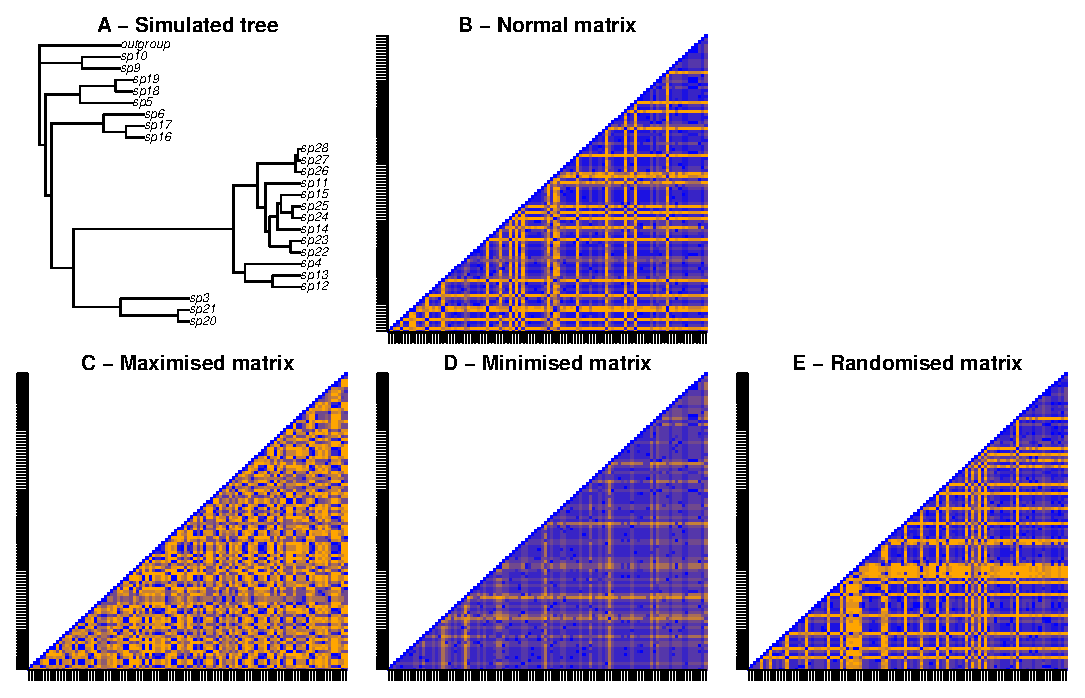
\includegraphics[width=1\textwidth]{Modif_matrix.eps}
\caption{Example illustration of the protocol for modifying matrices. The matrices represent the pairwise character differences for 100 characters. Blue colours correspond to low character differences and orange colours correspond to high character differences. \textcolor{blue}{\textbf{A} - a random Birth-Death tree is simulated and used for generating the unperturbed matrix (\textbf{B}), characters in this matrix are then removed or duplicated to maximise (\textbf{C}) or minimise (\textbf{D}) character correlation; or to randomise characters (\textbf{E}). The differences between the characters is low in \textbf{C} (decreased compared to \textbf{A}) implying a maximised correlation between the characters. Conversely, the character differences is high in \textbf{D} (increased compared to \textbf{A}) implying a minimised correlation between the characters.}}
\label{Fig:modif_matrix}
\end{figure}

\subsection{Inferring topologies}
We inferred the topologies with both Bayesian inference and maximum parsimony using MrBayes \citep[v3.2.6;][]{Ronquist2012mrbayes} and PAUP* \citep[v4.0a151;][]{swofford2001paup} respectively.
For both methods, we used the arbitrarily chosen outgroup in the simulations to root our trees (the first taxon in the taxa list).
The maximum parsimony inference was run using a heuristic search with random sequence addition replicate 100 times with a limit of $5\times10^6$ rearrangements per replicates.

Bayesian inference was run using an M\textit{k} model with ascertainment bias and four discrete gamma rate categories (M\textit{kv} $4\Gamma$) with an variable rate prior an exponential (0.5) shape.
\textcolor{blue}{We’ve used the Mk model with ascertainment bias (Mkv) to correct for the fact that no invariant characters were present in the matrix (as is often the case with morphological data) allowing the model to estimate the correct evolutionary rates (see above).
We used four discrete character rates categories making the assumption that each character has an independent $\frac{1}{4}$ chance to be in the $1^{st}$, $2^{nd}$, $3^{rd}$ or $4^{th}$ quartile of the rate distribution.
Finally we allowed that the average rate of this distribution ($\alpha$) is drawn from an exponential distribution (with a mean of 0.5) in every iteration of the MCMC allowing an efficient exploration of the parameter space.}
The MCMC was ran over two runs of 6 chains each for a maximum of $1\times10^9$ generations with a sampling every 200 generations with an automatic stop if the average standard deviation of split frequency (ASDSF) fell below 0.01.
\textcolor{blue}{We used this method to diagnose when the 12 chains reached a similar region in the parameter space. In other words, we considered that when the differences in solutions between the chains reaches a stabilised solution independently (ASDSF $<0.01$), then the MCMC converged on the ``correct'' inference.}
Due to cluster hardware requirements and to save some time, when chains didn't converge and the runs exceeded 5GB each, we aborted the MCMC and computed the consensus tree from the unconverged chains.
In practice, these few MCMC got stuck at an ASDSF around (but not below) 0.01.

A majority rule tree was then calculated for both maximum parsimony and Bayesian trees (discarding the 25\% first trees).
The 1440 tree inferences took around one CPU century on the Imperial College High Performance Computing Service \citep[2-3GHz clock rate;][]{HPC} and the Australian QRIScloud Awoonga clusters (3Ghz).

\subsection{Comparing topologies}
We compared the topologies using the same approach as in \cite{Guillerme2016146}: we measured both the Robinson-Foulds distance (\textcolor{blue}{the differences in clade compositions}, \citealt{RF1981}) and the triplets distance (\textcolor{blue}{the differences in tips positions}; \citealt{dobson1975triplets}) between the trees inferred from the maximised correlation, minimised correlation and randomised matrices and the tree inferred from the unperturbed matrix (Figs \ref{Fig:RF_results_best} and \ref{Fig:Tr_results_best} and supplementary materials 3 Figs 10 and 11).
Note that we are not comparing the trees to the starting tree used to simulate the matrices.
This is because, first, in biology, this tree is always unknown; and second, our objective is to measure the direct effect of character correlation approximated by the difference in topology between the unperturbed,  maximised correlation and minimised correlation trees.

The metric scores were calculated using the \texttt{TreeCmp} javascript \citep{Bogdanowicz2012}.
The measurements were then standardised using the Normalised Tree Similarity metric \citep[$NTS$; centering and scaling the metric score to the number of taxa;][]{Bogdanowicz2012,Guillerme2016146}.
The normalised score for both metrics thus reflects two distinct aspects of tree topology: (1) the Normalised Robinson-Foulds Similarity ($NTS_{RF}$)  reflects the conservation of clades; and (2) the Normalised Triplets Similarity ($NTS_{Tr}$) reflects the position of taxa.

To measure the effect of character correlation, we used a combination of the Wilcoxon rank test with a Bonferonni-Holm corrections \citep{holm1979simple} and a the probability of overlap between two distributions \citep[the Bhattacharyya Coefficient: $BC$;][]{Bhattacharyya}.
The resulting full simulation was 2TB in size so is not shared here (though the parameters are).
However, the resulting consensus trees on which the topological differences are calculated are available at \url{https://figshare.com/s/7a8fde8eaa39a3d3cf56}.

%---------------------------------------------
%
%       RESULTS
%
%---------------------------------------------
\section{Results}

\begin{figure}[!htbp]
\centering
   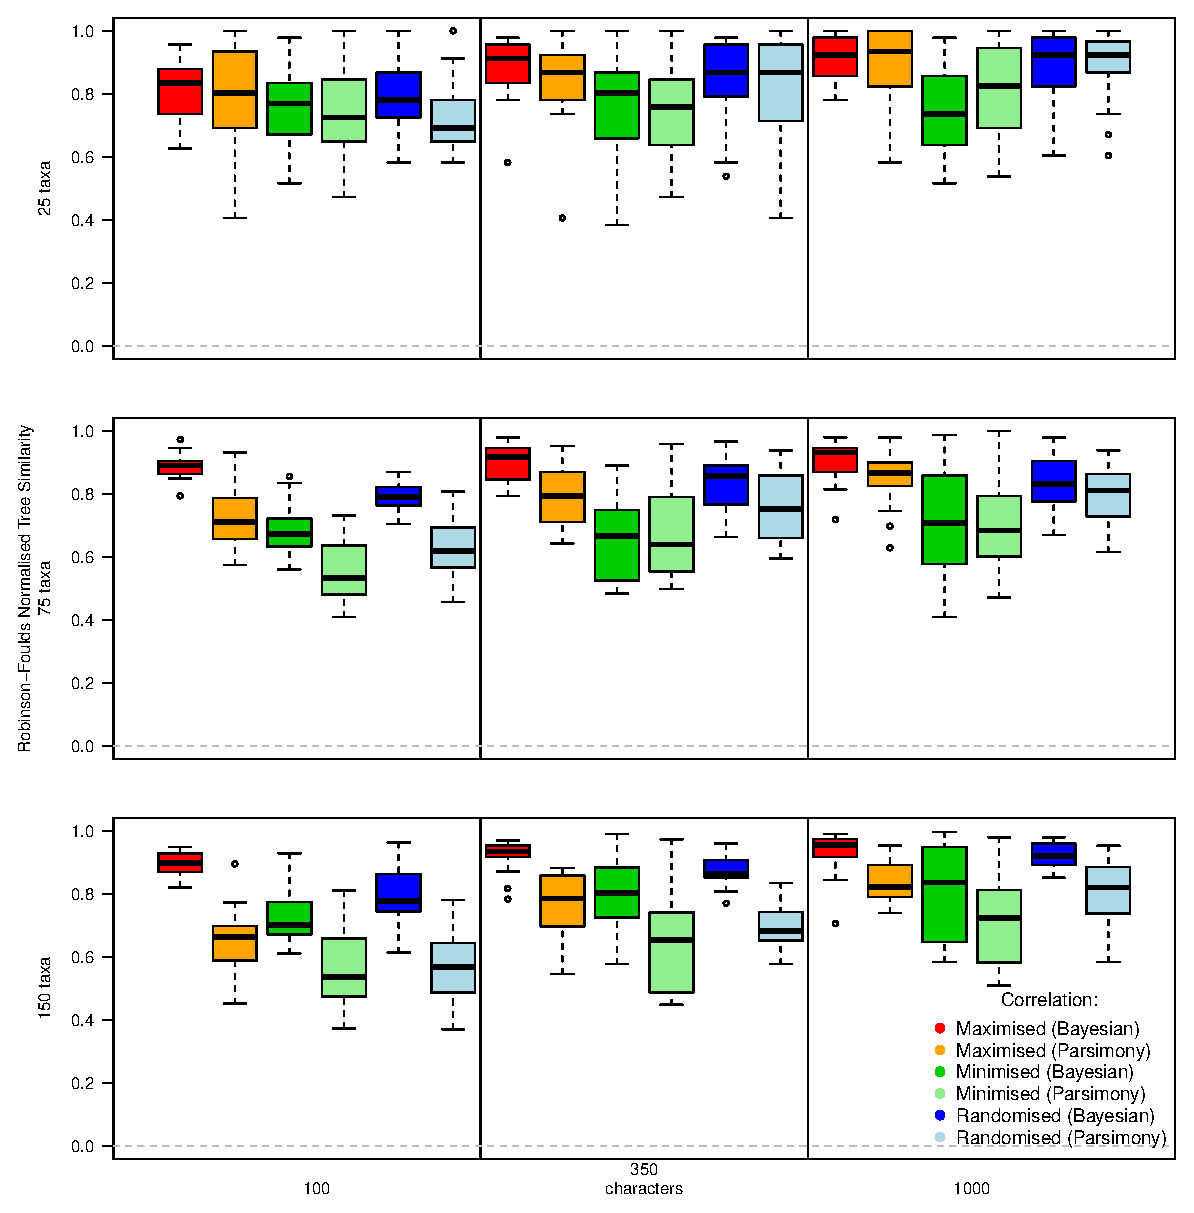
\includegraphics[width=1\textwidth]{RF_results_best.eps}
\caption{\small{Effect of character correlation on recovering the topology from the unperturbed matrix in terms of clade conservation ($NTS_{RF}$). The y axis represents the Normalised Tree Similarity using Robinson-Fould distance for matrices with 25, 75 and 150 taxa from top to bottom respectively. The x axis represents the different correlation scenarios and tree inference method with the maximised correlation in Bayesian (red) and under maximum parsimony (orange), the minimised correlation in Bayesian (dark green) and under maximum parsimony (light green) and the randomised correlation in Bayesian (dark blue) and under maximum parsimony (light blue) for matrices of 100, 350 and 1000 characters in the panels from left to right.}}
\label{Fig:RF_results_best}
\end{figure}

\begin{figure}[!htbp]
\centering
   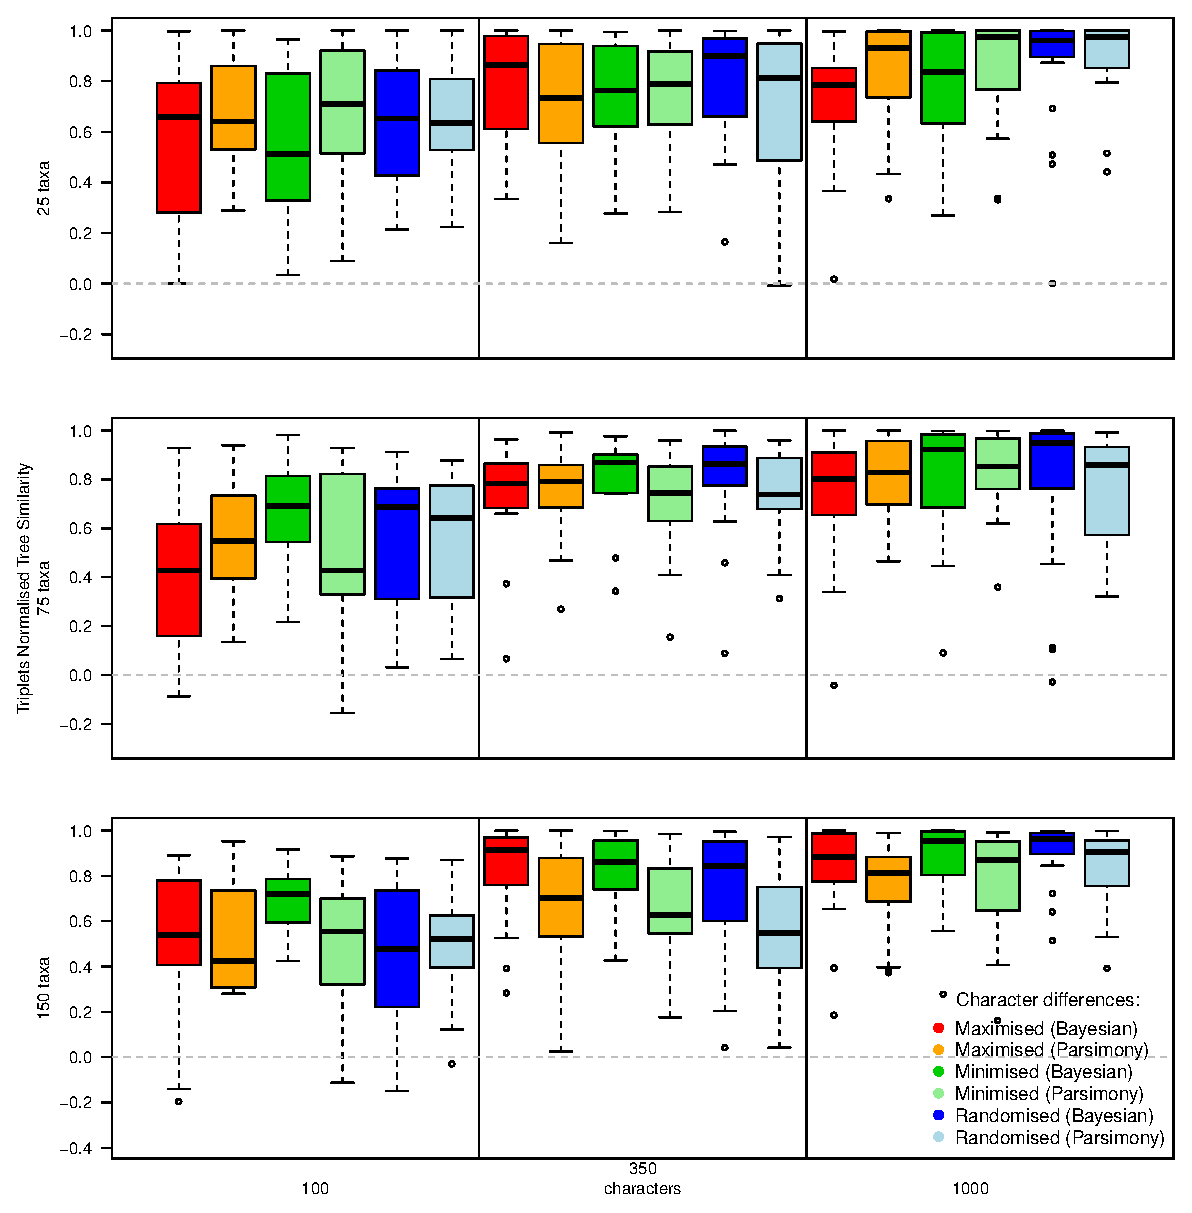
\includegraphics[width=1\textwidth]{Tr_results_best.eps}
\caption{Effect of character correlation on recovering the topology from the unperturbed matrix in terms of Triplets ($NTS_{Tr}$). The axis are identical to figure \ref{Fig:RF_results_best} but y axis represents the Normalised Tree Similarity using Triplets distance.}
\label{Fig:Tr_results_best}
\end{figure}

\subsection{Effect of character differences on topology}
\textcolor{blue}{The overall amount of character difference in a matrix has an effect of the ability to recover the topology from the unperturbed matrix when maximised character correlation leading to the smallest loss in phylogenetic information followed by randomising and minimising the character correlation} (see supplementary materials 3, Tables 3, 4 and 5).
There is a significant difference between all scenarios in terms of clade conservation ($NTS_{RF}$ - Table \ref{Tab_pooledscenarios_test}).
However, there is no difference in terms of taxon displacement between the three scenarios ($NTS_{Tr}$ - Table \ref{Tab_pooledscenarios_test}).

% latex table generated in R 4.1.3 by xtable 1.8-4 package
% Thu Mar 24 14:24:05 2022
\begin{table}[ht]
\centering
\begin{tabular}{llr|rr}
  \hline
metric & test & bhatt.coeff & statistic & p.value \\ 
  \hline
RF & maximised vs. minimised & 0.848 & 97587.500 & \textbf{0.000} \\ 
   & maximised vs. randomised & \textbf{0.954} & 80382.500 & \textbf{0.000} \\ 
   & minimised vs. randomised & 0.941 & 44161.000 & \textbf{0.000} \\ 
  Tr & maximised vs. minimised & \textbf{0.992} & 68919.500 & 0.839 \\ 
   & maximised vs. randomised & \textbf{0.982} & 64222.500 & 1.000 \\ 
   & minimised vs. randomised & \textbf{0.980} & 60447.000 & 0.713 \\ 
   \hline
\end{tabular}
\caption{Differences between the Normalised Tree Similarities in terms of clade conservation (Robinson-Foulds distances - RF) and taxa displacement (Triplets - Tr) for each maximised, minimised and randomised character correlation. Bhatt.coeff is the Bhattacharrya Coefficient (probability of overlap), the statistic and the p.value are from a non-parametric Wilcoxon test (with Bonferonni-Holm correction).} 
\label{Tab_pooledscenarios_test}
\end{table}


\subsubsection{Number of characters}
The effect of the character difference affects clade conservation ($NTS_{RF}$) only over large differences in number of characters (100 \textit{vs.} 1000 - Table \ref{Tab_pooledscharacters_test}).
For closer differences between characters numbers (100 \textit{vs.} 350 and 350 \textit{vs.} 1000), Wilcoxon tests showed clear differences ($p = 0$) but with high distribution overlap ($BC > 0.96$).
Regarding taxon displacements ($NTS_{Tr}$), there was an effect of the number of characters although the with a high distribution overlap between 350 and 1000 characters (Table \ref{Tab_pooledscharacters_test}).

% latex table generated in R 3.5.3 by xtable 1.8-3 package
% Tue Apr 16 16:07:59 2019
\begin{table}[ht]
\centering
\begin{tabular}{llr|rr}
  \hline
metric & test & bhatt.coeff & statistic & p.value \\ 
  \hline
RF & c100:c350 & \textbf{0.965} & 48263.500 & \textbf{0.000} \\ 
   & c100:c1000 & 0.914 & 37714.500 & \textbf{0.000} \\ 
   & c350:c1000 & \textbf{0.976} & 53138.000 & \textbf{0.000} \\ 
  Tr & c100:c350 & 0.929 & 40253.000 & \textbf{0.000} \\ 
   & c100:c1000 & 0.826 & 27923.000 & \textbf{0.000} \\ 
   & c350:c1000 & \textbf{0.957} & 48164.500 & \textbf{0.000} \\ 
   \hline
\end{tabular}
\caption{Difference between the pooled number of characters. Bhatt.coeff is the Bhattacharrya Coefficient (probability of overlap), the statistic and the p.value are from a non-parametric wilcoxon test (with Bonferonni-Holm correciton)} 
\label{Tab_pooledscharacters_test}
\end{table}


\subsubsection{Number of taxa}
Similar to the effect of number of characters on character difference, the number of taxa seems to have only a marginal effect.
A low number of taxa (25) resulted in significant differences with both 75 or 150 taxa in $NTS_{RF}$ (Table \ref{Tab_pooledstaxa_test}) but no differences between 75 and 150 taxa for $NTS_{Tr}$ (Table \ref{Tab_pooledstaxa_test}).
The significant differences have to be contrasted with still high probabilities of overlaps for each $NTS_{RF}$ and $NTS_{Tr}$ distributions for every number of taxa (Table \ref{Tab_pooledstaxa_test}).

% latex table generated in R 3.5.3 by xtable 1.8-3 package
% Tue Apr 16 16:08:34 2019
\begin{table}[ht]
\centering
\begin{tabular}{llr|rr}
  \hline
metric & test & bhatt.coeff & statistic & p.value \\ 
  \hline
RF & t25:t75 & 0.949 & 79945.000 & 0.000 \\ 
   & t25:t150 & 0.954 & 75906.000 & 0.000 \\ 
   & t75:t150 & 0.984 & 60328.000 & 0.654 \\ 
  Tr & t25:t75 & 0.960 & 72814.000 & 0.024 \\ 
   & t25:t150 & 0.961 & 72716.000 & 0.027 \\ 
   & t75:t150 & 0.980 & 64637.000 & 1.000 \\ 
   \hline
\end{tabular}
\caption{Difference between the pooled number of taxa. Bhatt.coeff is the Bhattacharrya Coefficient (probability of overlap), the statistic and the p.value are from a non-parametric wilcoxon test (with Bonferonni-Holm correciton)} 
\label{Tab_pooledstaxa_test}
\end{table}


\subsection{Effect of character differences on the inference method}
Regarding the inference method, there is a significant difference in clade conservation between Bayesian and maximum parsimony (\textit{p} = 0 Table \ref{Tab_pooledsmethods_test}) but not in terms of individual taxon placements (\textit{p} = 0.041 but $BC > 0.95$; Table \ref{Tab_pooledsmethods_test}).

% latex table generated in R 3.4.4 by xtable 1.8-2 package
% Tue Mar 27 14:03:14 2018
\begin{table}[ht]
\centering
\begin{tabular}{llr|rl}
  \hline
metric & test & bhatt.coeff & statistic & p.value \\ 
  \hline
RF & bayesian:parsimony & 0.891 & 579437.500 & \textbf{0} \\ 
  Tr & bayesian:parsimony & \textbf{0.984} & 470621.500 & 0.084 \\ 
   \hline
\end{tabular}
\caption{Difference between the pooled methods. Bhatt.coeff is the Bhattacharrya Coefficient (probability of overlap), the statistic and the p.value are from a non-parametric wilcoxon test (with Bonferonni-Holm correciton)} 
\label{Tab_pooledsmethods_test}
\end{table}


\subsection{Combined effects of taxa, characters and correlation on topology}
When looking at the combined effect of each parameter, the maximised, minimised or randomised correlation scenarios $NTS_{RF}$ and $NTS_{Tr}$ never overlap ($BC < 0.95$ - supplementary material 3, tables 16 and 17).
When comparing the distribution using the Wilcoxon ranked tests, there was no clear differences between tree similarity of differencing numbers of taxa, characters, tree correlation, or tree inference method for the taxon displacement metric ($NTS_{Tr}$ - supplementary material 3, tables 21 and 22).
In terms of clade conservation ($NTS_{RF}$), however, maximised and minimised correlation scenarios produced nearly always consistently different topologies using Bayesian inference (apart for the matrices with 25 taxa and 100 and 350 characters and the matrices with 150 taxa and 350 characters) but not using parsimony (only the matrices with 75 taxa and 100 or 350 characters produced different $NTS_{RF}$ distributions - supplementary material 3, tables 19 and 20).

\section{Discussion}

\subsection{Effect of character differences on topology}
We find that there is a significant influence of morphological character correlation on inferring tree topology.
When characters are correlated, matrices convey a strong (but potentially misleading) phylogenetic signal since characters are more likely to agree with each other and conversely, when characters are uncorrelated, one could expect them to convey a weaker phylogenetic signal with a high amount of characters giving a conflicting signal (homoplasy).
Throughout our simulation, the ``minimised'' character difference scenario (i.e. increased correlation) tended to result in trees slightly closer to the ``true'' tree and the ``maximised'' character difference scenario led to slightly worse trees (Fig. \ref{Fig:RF_results_best}).
These results suggest that, in matrices with high character differences, bootstrapping or other data randomisation methods can effectively improve the ability to recover the correct topology.

However, this effect of increasing or reducing character difference did not appear to affect taxon placement ($NTS_{Tr}$) for which the confidence intervals overlapped too much to be able to discern clear statistical differences (Fig.\ref{Fig:Tr_results_best}).
Furthermore, these results needs to be contrasted with the fact that the trees generated by the ``minimised'' character difference scenario do not appear better resolved (towards any topology) than the other scenarios (see supplementary material 3, Figs 12, 13 and 14).
Furthermore, fewer characters were replaced, on average, in the ``minimised'' matrices compared to both the ``maximised'' and ``randomised'' matrices (supplementary material 3, Figs 7, 8 and 9) although this did not change the way the average character differences varied across the matrices (supplementary material 3, Figs 4, 5 and 6).
This suggest that character difference can be decreased with a smaller amount of characters replacements than increasing it.

\subsubsection{Number of characters and taxa}
We found an effect of the number of characters on the ability to recover the ``best'' topology with different levels of character correlations only between the two extreme number of characters (100 and 1000; Tables \ref{Tab_pooledscharacters_test}).
This is expected since a higher number of characters can result in better topologies with a higher probability of ``noisy'' signal to cancel (\textit{c.f.} in smaller matrices).
While matrices with more characters or taxa tended to be better resolved than matrices with fewer characters or taxa, the effect of character correlation on topology is independent of the size of the matrix (Tables \ref{Tab_pooledscharacters_test} and \ref{Tab_pooledstaxa_test}).
This can be explained partly by our method of comparing trees using the Normalised Tree Similarity \citep[$NTS$;][]{Bogdanowicz2012} which corrects for the fact that topological differences are proportional to the number of taxa considered.

\subsubsection{Effect of character differences on the inference method}
When considering the pooled effect of the tree inference method, we only detected a significant difference between the Bayesian and the maximum parsimony trees in terms of clade conservation but none in terms of taxa placement (Table \ref{Tab_pooledsmethods_test}).
The difference in the ability of each method to recover the ``correct'' topology has been recently discussed with some indications that Bayesian inference will outperform parsimony when analysing discrete morphological characters alone (\citealt{wrightbayesian2014,OReilly20160081,puttick2017uncertain}; but see \citealt{spencerefficacy2013,goloboff2017weighted}).
In this study, it is possible that our simulation protocol for generating the characters (using some M$k$-based characters) could slightly favour Bayesian inference over maximum parsimony, however, our protocol for selecting matrices \citep[using matrices with a $CI>0.26$;][]{OReilly20160081} could also favour maximum parsimony analysis.
It was however not the purpose of this study to compare the overall performance of both methods but rather to measure the effect of character correlation on each of those methods separately.

\subsection{Distinction between different character correlations}
Here we mention three different types of character correlations but evolutionary biologists are mainly interested in intra-organismal and evolutionary correlations (e.g. in evo-devo \citealt{goswami2006morphological}; or in macroevolution \citealt{fitzjohn2014much}).
These two types of correlations can only be studied \textit{a posteriori} with a phylogenetic hypothesis and should not be used \textit{a priori} as a criterion to select characters (to avoid creating circular and biased reasoning).
This creates a trade-off between: (1) coding fewer characters (stochastically reducing \textit{a priori} correlation) but making the \textit{a posteriori} correlation more dependent on the coding;
and (2) coding more characters (increasing \textit{a priori} dependence) but allowing the \textit{a posteriori} correlation to be less dependent on the coding correlations.

Intra-organismal and evolutionary correlations are present in our simulations although they were not explicitly modelled:
(1) evolutionary correlation is implied by simulating the characters using Birth-Death trees;
and (2) intra-organismal correlation is present in the matrices for the characters randomly simulated but sharing similar evolutionary simulation regimes.
However, the effect of these sources of correlation was out of the scope of this study and would have required \textit{a posteriori} changes to the matrices \citep{Lande1983,Maddison1990,Pagel1994}.

\subsection{Potential applications}
Effectively, our simulation protocol bootstraps our data ``with bias''.
In the ``randomised'' scenarios the data is simply randomly bootstrapped.
However, in the ``minimised'' and ``maximised'' scenario, we remove the characters with the lowest/highest overall character difference.
For example, in the ``maximised'' scenario, we randomly remove some characters that are strongly correlated with each other and randomly resample from the characters left.

In rather small matrices (25 $\times$ 100), there was no significant difference in terms of recovering the right topology when maximising or randomising the character differences.
Since many discrete morphological matrices are of similar size \citep{guillerme2016assessment} a simple bootstrap re-sampling
will be sufficient to obtain a robust topology.
In matrices with more taxa, however, the ``minimised'' scenario resulted in better topological recovery.
Applying this type of bootstraps that minimised character difference by biasing the random sampling could thus help in understanding which characters generate more homoplasy, which nodes in the tree are conflictual or which clades might be most dependent on highly correlated characters. 
Overall, we suggest measuring (and reporting) the levels of character difference in a matrix to help understand potential caveats in the data.
In fact, regions of the matrix where characters have a consistent low difference can reflect that they are coding for the same information.

\subsection{Limitations}
First, simulating evolutionary history is complex.
Not only because the models we're using to infer phylogenies are ever-improving \citep[e.g.][]{heath2014fossilized,Wright01072016} but also because generalising morphological evolution across vastly different organisms is probably impossible \citep[see constrasted discussions from][]{GoloboffEmpirical,OReillyEmpirical}.
However, we do not compare the ``maximised'', ``minimised'' and ``randomised'' to the ``true'' tree but rather to the ``normal'' tree.
This allows us to reduce the caveats from our simulations on the effect of character correlation since we only compare the simulation end products to the other outputs rather than to the simulation inputs.
 
Second, comparing phylogenetic inference methods is not trivial.
As mentioned above, both maximum parsimony and Bayesian inference have similar outputs nut vastly differ in how optimality is measured.
There are also difficulties in summarising both methods with consensus trees \cite{oReilly2017efficacy}.
However, we want to point out again that here we are not comparing the methods to each other \textit{per se} but rather how they both, individually, react to an increase or decrease of correlated characters.


\subsection{Conclusion}
Correlation between characters can be induced through three main phenomena: intra-organismal relationships, selection-driven covariation or biases in coding the characters yet only the latter can be improved upon.
Useful best practices guidelines \citep[e.g.][]{Brazeau2011,simoes2017giant} and algorithms for dealing with different types of character correlations \citep[e.g. ][]{de2015parsimony,BrazeauNA} already exist.
However, with the expansion of dataset size \citep[e.g.][> 1000 characters]{nithe2013,O'Leary08022013}, we can expect the correlation between characters to increase stochastically.
Moreover, because phylogenetic inference software are unable to \textit{a priori} differentiate between these correlation types, it is important to understand to what extent topologies can be influenced by such bias.

We found that character correlation has a strong effect on recovering the correct topology: matrices with high character differences always performed more poorly at recovering the correct topology than trees with low or randomised character differences.
This is especially true in large matrices where we advise to reduce character difference by using bootstrapping with ``bias'' whereas this may not be major problem in modest size matrices (25 taxa; 100 to 350 characters).
However, in empirical datasets, if character difference is not driven by selection (e.g. pleiotropy) correlation is likely be cancelled out if the correlated characters are randomly distributed with respect to traits.
We recommend that all morphological phylogenetic analyses should report the level of character difference so that we can begin to detect and address the problem of coding dependence on inflating our confidence in our phylogenetic reconstructions.

\section{Data availability, repeatability and reproducibility}
The consensus trees are available on figshare at \url{https://figshare.com/s/7a8fde8eaa39a3d3cf56}.
The simulations are fully replicable following the explanations at \url{https://github.com/TGuillerme/CharactersCorrelation}.
The post-simulation analysis, tables and figures (reported in this manuscript) are fully reproducible see (\url{https://github.com/TGuillerme/CharactersCorrelation}).

\section{Funding}
European Research Council under the European Union’s Seventh Framework Programme (FP/2007–2013)/ERC Grant Agreement number 311092.

\section{Acknowledgements}
Calculations where done using the Imperial College London Cluster Services (doi: 10.14469/hpc/2232) and the Australian QRIScloud Awoonga cluster services. We thank Alberto Pascual Garcia for input in the design of the simulations protocol and Orlin Todorov for assistance with the computations. We also thank the three anonymous reviewers for there constructive and insightful comments.

\bibliographystyle{sysbio}
\bibliography{References}


\end{document}